%\documentclass[aspectratio=169]{beamer}
\documentclass[aspectratio=169,xcolor={table,dvipsnames,usenames}]{beamer}
\usefonttheme[onlymath]{serif}
\usepackage[brazilian]{babel}


\mode<presentation>
{
  \usetheme{Madrid}      % or try Darmstadt, Madrid, Warsaw, ...
  \usecolortheme{dolphin} % or try albatross, beaver, crane, ...
  \usefonttheme{default}  % or try serif, structurebold, ...
  \setbeamertemplate{navigation symbols}{}
  \setbeamertemplate{caption}[numbered]
  \setbeamertemplate{headline}{}
}

\usepackage{mathtools}
%\usepackage{amsthm}
\usepackage{amsmath}
%\usepackage{nccmath}
\usepackage{amssymb}
%\usepackage{amsfonts}
\usepackage{physics}
%\usepackage{dsfont}
%\usepackage{mathrsfs}
%\usepackage{slashed}    % Feynman slash notation, requires LuaLaTeX
%\usepackage[compat=1.1.0]{tikz-feynman}   % Feynman diagrams

%\usepackage{titling}
\usepackage{indentfirst}
%\usepackage[titletoc,title]{appendix}
%\renewcommand\appendixname{Apêndice}

\usepackage{bm}
%\usepackage{xcolor}
%\usepackage[dvipsnames]{xcolor}
\usepackage{cancel}

%\usepackage{xurl}
\usepackage{hyperref}
\usepackage{cite}

\usepackage{float}
\usepackage{graphicx}
\usepackage{tikz}
\usepackage{caption}
\usepackage{subcaption}

%%%%%%%%%%%%%%%%%%%%%%%%%%%%%%%%%%%%%%%%%%%%%%%%%%%

\newcommand{\eps}{\epsilon}
\newcommand{\vphi}{\varphi}
\newcommand{\cte}{\text{cte}}

\newcommand{\N}{\mathbb{N}}
\newcommand{\Z}{\mathbb{Z}}
\newcommand{\Q}{\mathbb{Q}}
\newcommand{\R}{\vb{R}}
\newcommand{\C}{\mathbb{C}}
\renewcommand{\S}{\vb{S}}
%\renewcommand{\H}{\s{H}}

\renewcommand{\a}{\vb{a}}
\renewcommand{\b}{\vb{b}}
\renewcommand{\d}{\dagger}
\newcommand{\up}{\uparrow}
\newcommand{\down}{\downarrow}
\newcommand{\hc}{\text{h.c.}}

\newcommand{\0}{\vb{0}}
\newcommand{\1}{\mathds{1}}
\newcommand{\E}{\vb{E}}
\newcommand{\B}{\vb{B}}
\renewcommand{\v}{\vb{v}}
\renewcommand{\r}{\vb{r}}
\renewcommand{\k}{\vb{k}}
\newcommand{\p}{\vb{p}}
\newcommand{\q}{\vb{q}}
\newcommand{\F}{\vb{F}}
\newcommand{\A}{\vb{A}}
\newcommand{\J}{\vb{J}}

\newcommand{\s}{\sigma}
\newcommand{\nn}[2]{\left\langle #1 , #2 \right\rangle}
\newcommand{\cc}[1]{\overline{#1}}
\newcommand{\Eval}[3]{\eval{\left( #1 \right)}_{#2}^{#3}}

\newcommand{\unit}[1]{\; \mathrm{#1}}

\newcommand{\n}{\medskip}
\newcommand{\e}{\quad \mathrm{e} \quad}
\newcommand{\ou}{\quad \mathrm{ou} \quad}
\newcommand{\virg}{\, , \;}
\newcommand{\ptodo}{\forall \,}
\renewcommand{\implies}{\; \Rightarrow \;}
%\newcommand{\eqname}[1]{\tag*{#1}} % Tag equation with name


%%%%%%%%%%%%%%%%%%%%%%%%%%%%%%%%%%%%%%%%%%%%%%%%%%%%%%%%%

\title[Supercondutividade não-convencional]{\LARGE{Supercondutividade não-convencional}}
\author[Mateus Marques]{
\large{Mateus Marques
}}
\date{\today}
%\titlegraphic{
\includegraphics[height=1.5cm]{logos/ifusp.png} \,\, 
\includegraphics[height=1.5cm]{logos/scientiavinces.png}}

\begin{document}

\begin{frame}
  \titlepage
\end{frame}

\begin{frame}{Supercondutores que vemos por aí}

\begin{figure}[H]
\centering
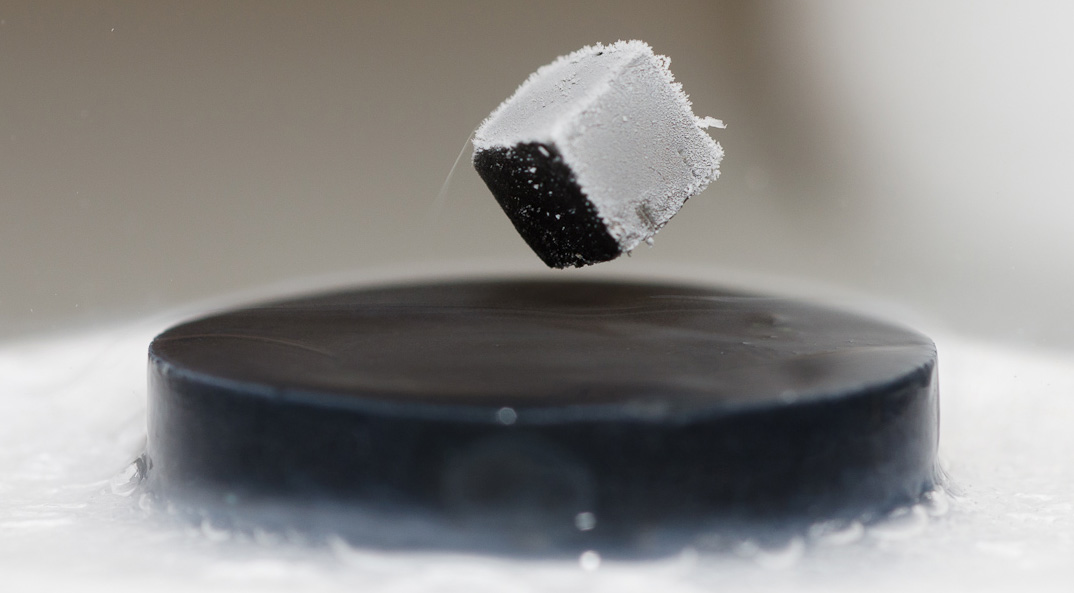
\includegraphics[width=0.7\textwidth]{fig/levitating.jpg}
\caption{Supercondutor de cuprato levitando sobre um ímã pelo efeito Meissner.}
\label{fig:levitating}
\end{figure}

\end{frame}

\begin{frame}{Diferentes supercondutores}

%\begin{itemize}
%\item BCS: Hg, Pb, NbGe$_3$, MgB$_2$.
%\end{itemize}

\begin{tabular}{ |p{3cm}||p{3cm}|p{3cm}|p{3cm}|  }
\hline
\multicolumn{4}{|c|}{Exemplos de supercondutores/superfluidos} \\
\hline
Supercondutor & Simetria & $T_c \approx$ & Categoria \\
\hline
Hg                   & s-wave   & $4.2   \, \text{K}$      & BCS \\
MgB$_2$              & s-wave   & $39    \, \text{K}$      & BCS \\
$^3$He               & p-wave   & $2.5   \, \text{mK}$     & Superfluido \\
Sr$_2$RuO$_4$        & p-wave   & $0.93  \, \text{K}$      & $-$ \\
YBCO                 & d-wave   & $93  \, \text{K}$        & Cuprato \\
BSCCO-2223           & d-wave   & $108   \, \text{K}$      & Cuprato \\
UPt$_3$              & f-wave   & $0.51  \, \text{K}$      & Heavy-Fermion \\
K$_3$C$_{60}$        & $-$      & $18    \, \text{K}$      & Orgânico  \\
LaO$_{1-x}$F$_x$FeAs & $-$      & $26    \, \text{K}$      & Ferro  \\
\hline
\end{tabular}

\end{frame}

\begin{frame}{Objetivos}

\begin{itemize}
\item Passar uma ideia introdutória de como generalizar a teoria BCS para estudar supercondutividade não-convencional.

\n\n

\item A inclusão de interações repulsivas e magnéticas causam anisotropia na função de gap.

\n\n

\item Entender a distinção básica das diferentes simetrias (jargão) s, p, d, f-wave.

\n\n

\item Existem mecanismos além dos fônons que geram interações atrativas?

\n\n

\item Foco específico nos cupratos e na simetria d-wave.
\end{itemize}



\end{frame}

\begin{frame}{Hipóteses da teoria BCS}

\begin{itemize}
\item O estado normal é um líquido de Fermi (metal).

\item Elétrons formam pares de Cooper pela interação atrativa mediada por fônons.

\n

\begin{figure}[H]
\centering
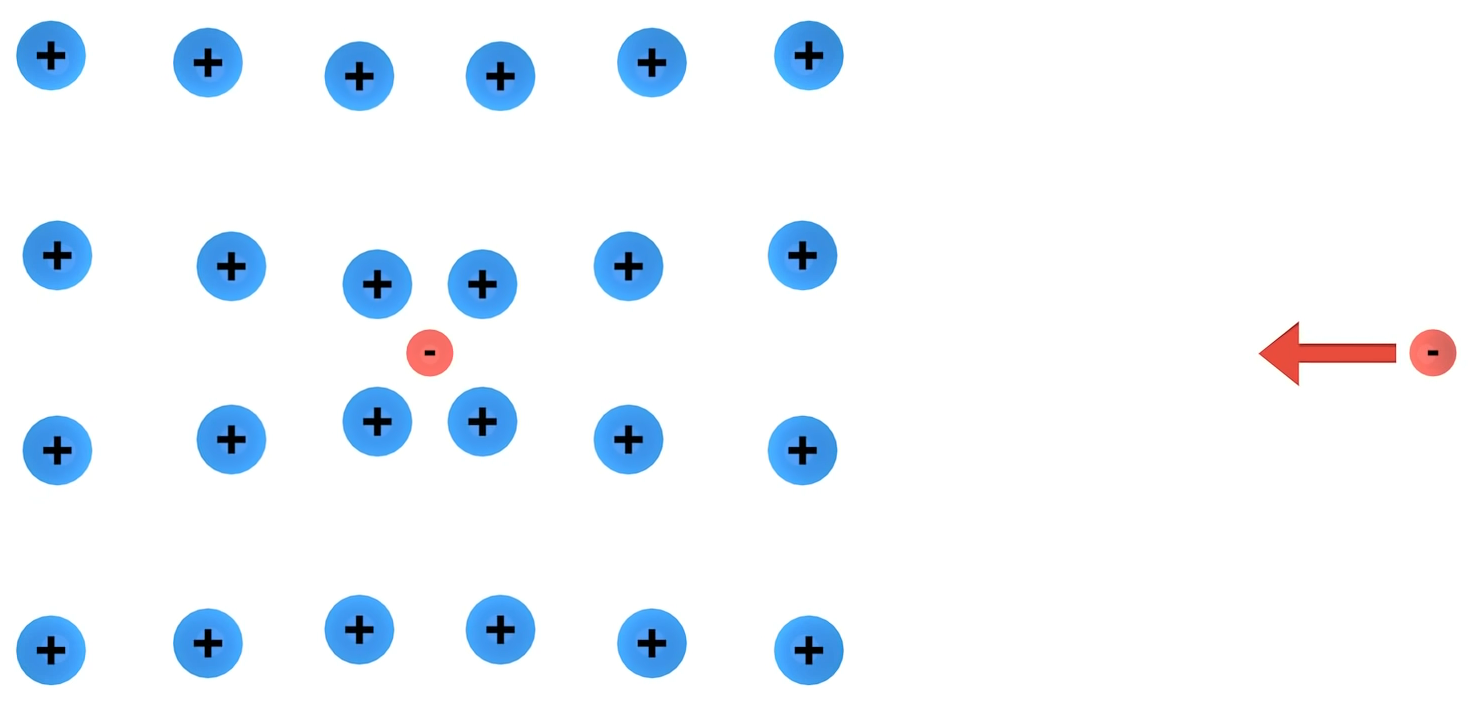
\includegraphics[width=0.5\linewidth]{fig/phonon.png}
\label{fig:phonon}
\end{figure}

\n

\item Os pares de Cooper são bósons e condensam num estado coerente, formando um superfluido carregado.

\item Dispersão $E_{\k} = \sqrt{\eps_{\k}^2 + \abs{\Delta}^2}$, onde o gap $\Delta$ não depende de $\k$ (esfericamente simétrico, ou s-wave).
\end{itemize}

\end{frame}

\begin{frame}{Equação do Gap}

Aproveitaremos parte do formalismo da teoria BCS. O raciocínio ainda se baseia na formação de pares de Cooper. Consideremos uma interação do tipo BCS
$$
H_I =
\frac{1}{V} \sum_{\k,\k'} V_{\k,\k'} (c_{\k\up}^\d c_{-\k\down}^\d) (c_{-\k'\down} c_{\k'\up}).
$$

Se definirmos o gap $\Delta_{\k} = \sum_{\k'} V_{\k,\k'} \ev{c_{-\k'\down} c_{\k'\up}}$ e aplicarmos o procedimento de campo médio $AB \simeq A\ev{B} + B\ev{A} - \ev{A}\ev{B}$, generalizamos a equação do gap
\begin{equation} \label{eq:gapeq}
\Delta_{\k} = - \sum_{\k'} V_{\k,\k'} \frac{\Delta_{\k'}}{2 E_{\k'}} \tanh(\frac{\beta E_{\k'}}{2}).
\end{equation}

Devido ao sinal negativo acima, se $V_{\k,\k'}$ não for sempre negativo, a função de gap $\Delta_{\k}$ poderá ser negativa em alguns pontos, de maneira a surgirem nós. Esse fenômeno acontece em várias classes de supercondutores: orgânicos, heavy-fermion, cupratos e baseados em ferro.

\end{frame}

\begin{frame}{Anisotropia}

Tendo em mente que queremos capturar os nós da função de gap, faremos considerações gerais sobre potenciais para estudar como a anisotropia pode surgir. Consideremos dois potenciais, um potencial repulsivo genérico
$$
V = \frac{1}{2} \sum_{\substack{\k_1,\k_2,\q \\ \s, \s'}} V_{\q} c_{\k_1+\q,\s}^\d c_{\k_2+\q,\s'}^\d c_{\k_2,\s'} c_{\k_1,\s},
$$
e um magnético
$$
V_{\text{mag}} = \sum_{i,j} J_{ij} \, \vb{S}_i \vdot \vb{S}_j = \frac{1}{2} \sum_{\q} J_{\q} \, \vb{S}_{-\q} \vdot \vb{S}_{\q}.
$$

\n

Analisaremos primeiro o potencial repulsivo $V$.

\end{frame}

\begin{frame}{Potencial repulsivo (1)}

Como estamos interessados na projeção nos pares de Cooper (momento total zero), consideramos que $\k_1 = -\k_2 = \k'$, $\k_1 + \q = -(\k_2 - \q) = \k$ e $\q = \k - \k'$. A interação resultante geral pode ser separada em termos de acordo com os spins
$$
V_{BCS} = \frac{1}{2} \sum_{\substack{\k,\k' \\ \s, \s'}} V_{\k-\k'} c_{\k\s}^\d c_{-\k\s'}^\d c_{-\k'\s'}c_{\k'\s} =
V_{BCS}^{\up\down} + V_{BCS}^{\up\up} + V_{BCS}^{\down\down}.
$$

Foquemos primeiramente no termo mais familiar
$$
V_{BCS}^{\up\down} = \sum_{\k,\k'} V_{\k-\k'} (c_{\k\up}^\d c_{-\k\down}^\d) (c_{-\k'\down} c_{\k'\up}) =
\sum_{\k,\k'} V_{\k-\k'} \Psi_{\k}^\d \Psi_{\k}.
$$

\end{frame}

\begin{frame}{Paridade e troca de spin}

Consideremos as propriedades de paridade $P$ e spin exchange $X$ da função de onda $F(\k)_{\alpha\beta} = \braket{\k\alpha,-\k\beta}{\k_P}$ do par de Cooper, definidas por
$$
P F(\k)_{\alpha\beta} = F(-\k)_{\alpha\beta},
$$
$$
X F(\k)_{\alpha\beta} = F(\k)_{\beta\alpha}.
$$

O operador de troca de spin distingue singletos $X = -1$ de tripletos $X = +1$.

\n

Obs: Lembremos que um par de spins $\ket{\up\down}$ não é singleto nem tripleto. De fato, o singleto é $(\ket{\up\down} - \ket{\down\up})/\sqrt{2}$ e o tripleto é composto por $(\ket{\up\down} + \ket{\down\up})/\sqrt{2}$, $\ket{\up\up}$ e $\ket{\down\down}$.

\n

Se aplicarmos $X$ e $P$ em $\braket{\k\alpha,-\k\beta}{\k_P}$ estaremos trocando os dois férmions que compõem o par, adquirindo uma fase $-1$. Portanto, $XP = -1$ no subespaço dos pares de Cooper.

\n

Temos então que pares com paridade par são singletos $(P,X) = (+, -)$ e com paridade ímpar são tripletos $(P,X) = (-,+)$.

\end{frame}

\begin{frame}{Singleto e tripleto}

Com autovalores dos operadores $P$ e $X$ em mente, podemos decompor a interação em partes simétrica (par, singleto) e antissimétrica (ímpar, tripleto):
$$
V_{BCS}^{\up\down} = \sum_{\k,\k'}
\Bigg[
\overbrace{\qty(\frac{V_{\k-\k'} + V_{\k+\k'}}{2})}^{V_{\k,\k'}^S} +
\overbrace{\qty(\frac{V_{\k-\k'} - V_{\k+\k'}}{2})}^{V_{\k,\k'}^T}
\Bigg] \Psi_{\k}^\d \Psi_{\k}.
$$

O primeiro termo acima espalha singletos e o segundo tripletos, representados por
$$
\Psi_{\k}^{S\d} = (c_{\k\up}^\d c_{-\k\down}^\d + c_{-\k\up}^\d c_{\k\down}^\d),
\quad \Psi_{\k}^{S\d} = +\Psi_{-\k}^{S\d},
$$
$$
\Psi_{\k}^{T\d} = (c_{\k\up}^\d c_{-\k\down}^\d - c_{-\k\up}^\d c_{\k\down}^\d),
\quad \Psi_{\k}^{T\d} = -\Psi_{-\k}^{T\d}.
$$

E escrevemos
$$
V_{BCS}^{\up\down} =
\frac{1}{4} \sum_{\k,\k'}
\qty[
V_{\k,\k'}^S \Psi_{\k}^{S\d} \Psi_{\k'}^{S} +
V_{\k,\k'}^T \Psi_{\k}^{T\d} \Psi_{\k'}^{T}
].
$$

\end{frame}

\begin{frame}{Potencial repulsivo (2)}

Os outros termos $V_{BCS}^{\up\up}$ e $V_{BCS}^{\down\down}$ somente envolvem tripletos, que interagem via $V_{\k,\k'}^T$. Se definirmos o vetor tripleto
$$
\va*{\Psi}_{\k}^T = \sum_{\alpha\beta} c_{\k\alpha}^\d \qty(\va*{\s} i \s_2)_{\alpha\beta} c_{-\k\beta}^\d =
\begin{cases}
\; \; \; \; c_{\k\down}^\d c_{-\k\down} - c_{\k\up}^\d c_{-\k\up}^\d \; , \quad (x) \\
\; i (c_{\k\down}^\d c_{-\k\down} + c_{\k\up}^\d c_{-\k\up}^\d), \quad (y) \\
\; \; \; \; c_{\k\up}^\d c_{-\k\down}^\d + c_{-\k\up}^\d c_{\k\down}^\d \; , \quad (z),
\end{cases}
$$
podemos representar as interações de spins paralelos de maneira compacta. No final obtemos
$$
V_{BCS} =
V_{BCS}^{\up\down} + V_{BCS}^{\up\up} + V_{BCS}^{\down\down} =
\frac{1}{4} \sum_{\k,\k'}
\qty(
V_{\k,\k'}^S \Psi_{\k}^{S\d} \Psi_{\k'}^S +
V_{\k,\k'}^T \va*{\Psi}_{\k}^{T\d} \va*{\Psi}_{\k'}^T
).
$$

\end{frame}


\begin{frame}{Observações sobre o potencial repulsivo}

\begin{itemize}
\item Ao estudarmos os harmônicos esféricos $Y_{\ell m}$ no contexto do átomo de Hidrogênio, vemos que a paridade está associada ao número quântico de momento angular orbital $\ell$, de maneira que $Y_{\ell m}(-\r) = (-1)^\ell Y_{\ell m}(\r)$.

\n

\item Pares de Cooper com função de onda de singleto envolvem $\ell = 0, 2, \ldots$ (s, d, $\ldots$ wave) e de tripleto envolvem valores ímpares $\ell = 1, 3, \ldots$ (p, f, $\ldots$ wave).

\n

\item Já que o potencial repulsivo $V_{BCS}$ se dissocia em interações de singleto e tripleto, podemos estudá-las separadamente. Em especial, só precisamos considerar o termo de tripleto $V^T_{\k,\k'}$ se estivermos interessados em descrever supercondutividade p-wave ou f-wave, por exemplo.

\n

\item Para um acoplamento somente de singleto, ficamos com a familiar
$$
V_{BCS} = \sum_{\k,\k'} V_{\k,\k'}^S (c_{\k\up}^\d c_{-\k\down}^\d) (c_{-\k'\down} c_{\k'\up}).
$$
\end{itemize}

\end{frame}

\begin{frame}{Interação magnética}

Analisamos agora a interação magnética (do tipo Heisenberg)
$$
V_{\text{mag}} = \frac{1}{2} \sum_{\q} J_{\q} \, \va*{S}_{-\q} \vdot \va*{S}_{\q} =
\frac{1}{2} \sum_{\k_1,\k_2,\q} J_{\q} c_{\k_1+\q,\alpha}^\d c_{\k_2-\q,\gamma}^\d
\qty(\frac{\va*{\s}}{2})_{\alpha\beta} \qty(\frac{\va*{\s}}{2})_{\gamma\delta} c_{\k_2\delta} c_{\k_1\beta},
$$
onde $J_{\q}$ é a interação efetiva dos spins. Por exemplo, para spins em uma rede quadrada interagindo só com primeiros vizinhos temos $J_{\q} = 2 J [\cos(q_x a) + \cos(q_y a)]$ (tight-binding).

\end{frame}

\end{document}
